\section{Evidence theory}

We aim to establish a measure of evidence for or against a proposition, employing two fuzzy measures: Belief and Plausibility.
\begin{definition}[\textit{Belief}]
    Belief is an estimate of the minimum probability that can be assigned to an element, considering the collected evidence.
\end{definition}
Belief is defined as follows:
\begin{itemize}
    \item $Bel:\wp (X) \rightarrow [0,1]$.
    \item $Bel(\varnothing)=0$ and $Bel(X)=1$.
    \item $Bel(A_1 \cup A_2 \cup \dots \cup A_n) \geq \sum_{j}Bel(A_j)-\sum_{j<k}Bel(A_j \cap A_k)+\dots+(-1)^{n+1}Bel(A_1 \cap A_2 \cap \dots \cap A_n)$
    \item $Bel(A)+Bel(\lnot A) \leq 1$.
\end{itemize}
\begin{definition}[\textit{Plausibility}]
    Plausibility is an estimate of the maximum probability that can be assigned to an element, considering the collected evidence. 
\end{definition} 
Plausibility is defined as follows:
\begin{itemize}
    \item $Pl:\wp (X) \rightarrow [0,1]$.
    \item $Pl(\varnothing)=0$ and $Pl(X)=1$.
    \item $Pl(A_1 \cap A_2 \cap \dots \cap A_n) \geq \sum_{j}Pl(A_j)-\sum_{j<k}Pl(A_j \cup A_k)+\dots+(-1)^{n+1}Pl(A_1 \cup A_2 \cup \dots \cup A_n)$
    \item $Pl(A)+Pl(\lnot A) \geq 1$.
\end{itemize}

\paragraph*{Applications}
Evidence theory finds application when multiple sources of knowledge exist, and the basic probability assignment is distributed across different sets of statements or intervals. 
In such cases, we can utilize the characteristics of evidence theory to accumulate basic probability assignments and combine them to assess upper and lower bounds for the probability of a single statement. 
Evidence theory implies that: 
\begin{itemize}
    \item There's no need to obtain a precise measurement from a knowledge source or experiment if it's not realistic or feasible.
    \item The principle of insufficient reason is not imposed. 
        Statements can be made about the likelihood of multiple events together without making assumptions about the probabilities of individual events under ignorance.
    \item The axiom of additivity is not imposed. 
        The measures can have the following properties:
        \begin{itemize}
            \item Add up to exactly one, which corresponds to a traditional probabilistic representation.
            \item Add up to less than one (sub-additive case), indicating incompatibility between multiple sources of information providing conflicting data.
            \item Add up to more than one (super-additive), suggesting a cooperative effect between multiple sources of information, such as multiple sensors providing the same information.
        \end{itemize}
\end{itemize}

\paragraph*{Information sources}
Given five sources ($A, B, C, D, E$ with $A$ as the target) of information, four cases can arise:
\begin{itemize}
    \item Conflict: in this scenario, each source provides evidence for disjoint sets.
        \begin{figure}[H]
            \centering
            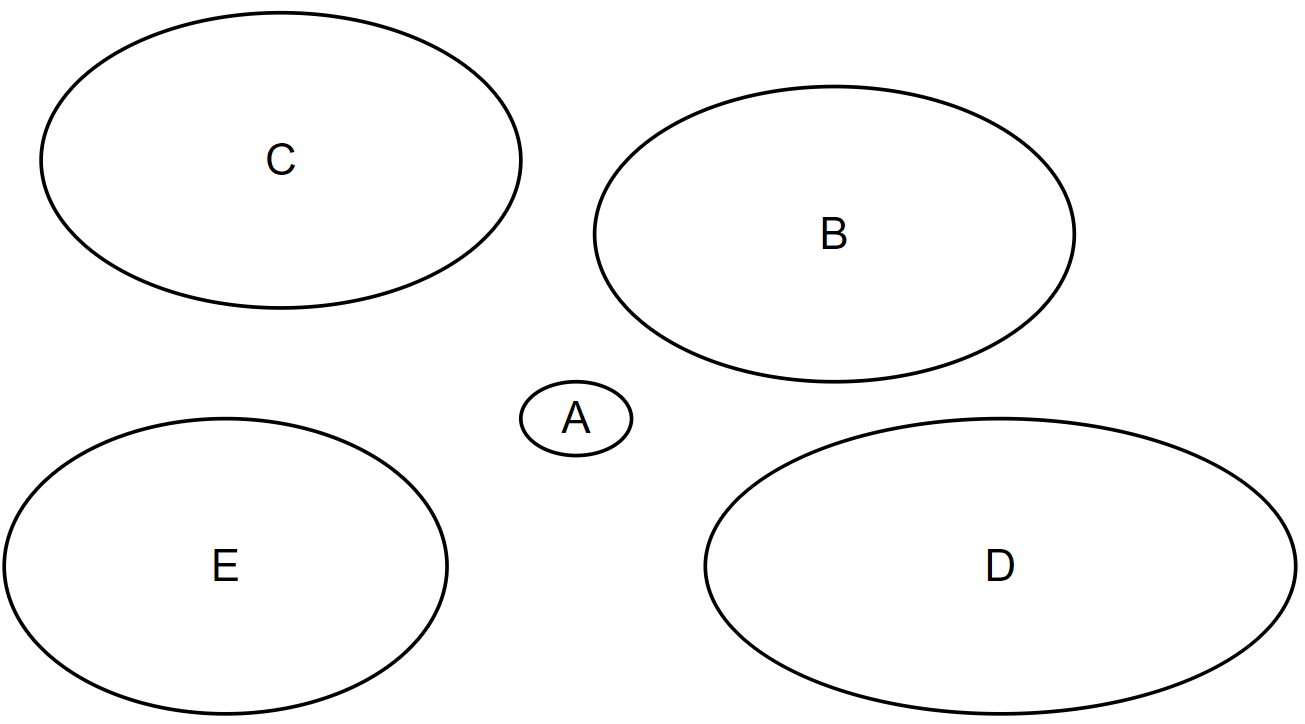
\includegraphics[width=0.5\linewidth]{images/conflict.png}
        \end{figure}
    \item Consonance: sources provide some evidence on nested sets, converging on the target.
        \begin{figure}[H]
            \centering
            
\includegraphics[width=0.5\linewidth]{images/consonance.png}
        \end{figure}
    \item Arbitrary: in the arbitrary case, each source provides evidence for sets, but only some of them include the target hypothesis.
        \begin{figure}[H]
            \centering
            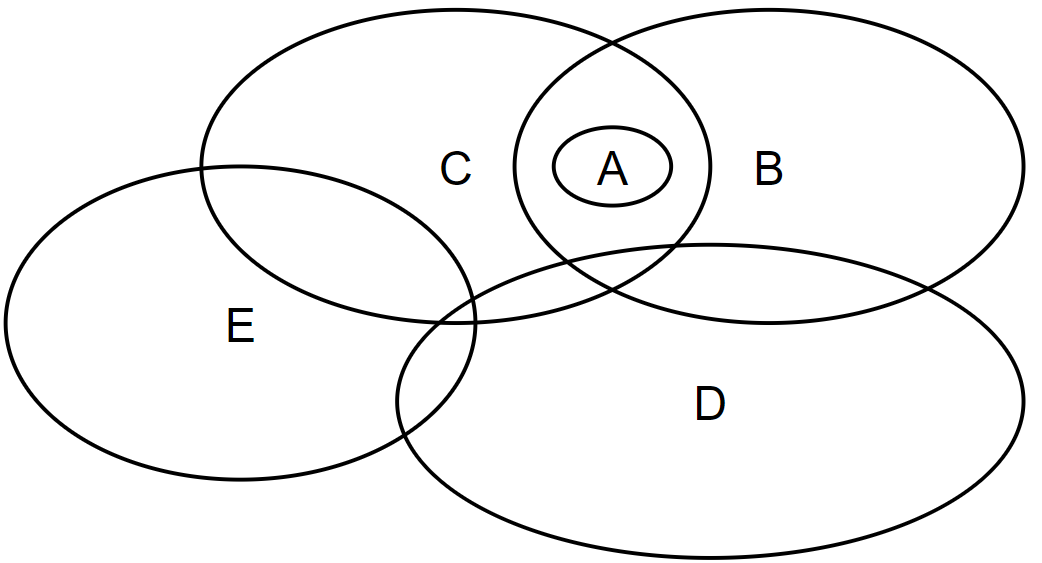
\includegraphics[width=0.5\linewidth]{images/arbitrary.png}
        \end{figure}
    \item Consistent: in this situation, all sources provide evidence for sets that include the same hypothesis.
        \begin{figure}[H]
            \centering
            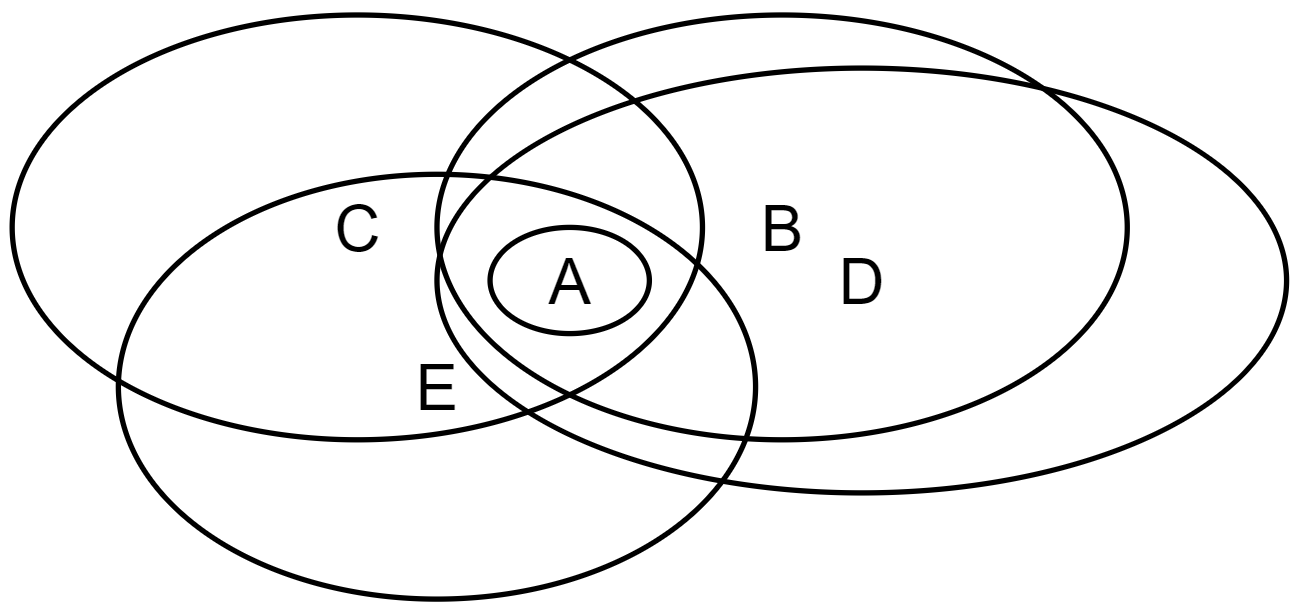
\includegraphics[width=0.5\linewidth]{images/consistent.png}
        \end{figure}
\end{itemize}

\paragraph*{Combining probability assignment}
To combine the basic probability assignments, the Dempster rule of combination can be used:
\[m_{1,2}(A)=\dfrac{\sum_{B \cap C=A}m_1(B)m_2(C)}{1-K}\]
Where $K$ is the basic probability mass associated with conflict. 
The role of $K$ in the denominator has the effect of completely ignoring conflict and attributing any probability mass associated with conflict to the null set. 
The value of this variable is determined by:
\[K=\sum_{B \cap C=O}m_1(B)m_2(C)\]
\begin{example}
    Let's consider the discovery of an old painting strongly resembling paintings by Raphael. 
    This discovery raises various questions about the painting's status. 
    We have three questions:
    \begin{enumerate}
        \item Is the discovered painting a genuine painting by Raphael?
        \item Is the discovered painting a product of one of Raphael's many disciples?
        \item Is the discovered painting a counterfeit?
    \end{enumerate}
    Assume that two experts conducted careful examinations of the painting and provided us with basic assignments $m_1$ and $m_2$. 
    Using the introduced formulas, we can compute the plausibility and belief of all the subsets of hypotheses.
\end{example}